\section{Establishing the Double Zeroes Property}

The way we prove that $a$ and $b$ have double zeroes at $E_8$ lattice points with norm $> \sqrt{2}$ (or at normalised $E_8$ lattice points with norm $> 1$) is by expressing the functions $a\rad$ and $b\rad$ as products of the $\sin^2$ function and another function, expressed as an integral.

\begin{wrapfigure}[7]{r}{0.4\linewidth}
    \vspace{-0.7em}
    \centering
    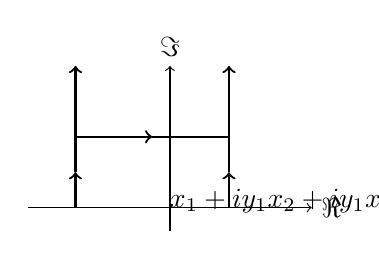
\begin{tikzpicture}[scale=1.5]
        % Axes
        \draw[->] (-1.2,0) -- (1.2,0) node[right] {$\Re$};
        \draw[->] (0,-0.2) -- (0,1.2) node[above] {$\Im$};
    
        % Contours
        \draw[thick, ->] (-0.8, 0) -- (-0.8,0.3);
        \draw[thick, ->] (-0.8,0.3) -- (-0.8, 1.2);
        \draw[thick, ->] (0.5, 0) -- (0.5,0.3);
        \draw[thick, ->] (0.5,0.3) -- (0.5, 1.2);
        \draw[thick, ->] (-0.8, 0.6) -- (-0.15, 0.6);
        \draw[thick] (-0.15, 0.6) -- (0.5, 0.6);
    
        % Points of interest
        \labelledpoint{-0.8}{0}{-0.4}{-0.8}{$x_1 + iy_1$}
        \labelledpoint{0.5}{0}{0.4}{-0.8}{$x_2 + iy_1$}
        \labelledpoint{-0.8}{0.6}{-0.8}{-0.3}{$x_1 + iy_2$}
        \labelledpoint{0.5}{0.6}{0.8}{-0.3}{$x_2 + iy_2$}
    \end{tikzpicture}
    \caption{Visualising the contours in \Cref{Ch4:Thm:CauchyGoursat_Unbounded}.}  
\end{wrapfigure}

The strategy to prove these two equalities will be to perform a change of contours using a version of the Cauchy-Goursat Theorem and use the relations and transformation rules between the $\phi$- and $\psi$-functions to combine integrals so that the result is exactly $a\rad$ or $b\rad$.

The version of the Cauchy-Goursat Theorem we use is the following.

\begin{boxtheorem}[Cauchy-Goursat for Unbounded Contours]\label{Ch4:Thm:CauchyGoursat_Unbounded}
    Suppose $f : \C \to \C$ is a function such that $f(z) \to 0$ as $\Im(z) \to \infty$. Then, for all $x_1, y_1, x_2, y_2 \in \R$, if $f$ is holomorphic at $z$ for all $z \in \C$ with $x_1 < \Re(z) < x_2$ and $y_1 < \Im(z)$, then
    \begin{align*}
        \int_{x_1 + iy_1}^{x_1 + i\infty} f(z) \, \diff{z}
        = \int_{x_1 + iy_1}^{x_1 + iy_2} f(z) \, \diff{z}
        + \int_{x_1 + iy_2}^{x_2 + iy_2} f(z) \, \diff{z}
        + \int_{x_2 + iy_2}^{x_2 + i\infty} f(z) \, \diff{z}
    \end{align*}
\end{boxtheorem}

We discuss the informal and formal proofs of this theorem in \Cref{Ch5:Sec:Cauchy-Goursat}.

For each eigenfunction, we begin by estimating certain quantities to show that the integrals in their alternate representation converge. We then prove that they satisfy the conditions of \Cref{Ch4:Thm:CauchyGoursat_Unbounded}. We will conclude by applying \Cref{Ch4:Thm:CauchyGoursat_Unbounded} and manipulating expressions.

\subsection{The $+1$-Eigenfunction}

We begin by defining the integral by which we represent $a\rad$.

\begin{boxdefinition}[Alternate Representation of $a$]
    Define $d\rad : \R \to \C$ by
\end{boxdefinition}

\subsection{The $-1$-Eigenfunction}